\section{Jan Vladislav}

\noindent
Vlastním jménem Ladislav Bambásek, je český básník a překladatel. Narodil se v Hlohovci na Slovensku v české rodině poštovního úředníka, bývalého legionáře. Roku 1939 odešel s rodinou do Čech a o tři roky později složil maturitu na gymnáziu v Poličce. Po válce studoval na Karlově univerzitě v Praze a dva semestry také v Grenoblu srovnávací dějiny literatury.

Vydal dvě knížky vlastní poezie a první výbor ze Shakespearových Sonetů, ale po únoru 1948 byl z politických důvodů z univerzity vyloučen a většina nákladu jeho třetí básnické knihy \textit{Hořící člověk} skončila v stoupě. Poté mohl v literatuře působit už jen pouze jako překladatel, případně autor knih pro mládež. Překládal a předmluvami nebo doslovy doprovázel zejména klasickou, moderní a lidovou poezii z angličtiny, francouzštiny, italštiny, němčiny, rumunštiny, ruštiny a ukrajinštiny a s jazykovou pomocí odborníků také z čínštiny a japonštiny. Jeho původní poezie zůstavala v rukopisech.

V roce 1968 se podílel na vzniku \textit{Kruhu nezávislých spisovatelů} a mohl konečně ukončit studia na FF UK doktorátem z filozofie.

Za normalizace byl znovu zbaven možnosti publikovat. Založil samizdatovou edici \textit{Kvart}, kde vyšlo přes 120 titulů, mezi nimi i několika svazků jeho vlastních básní, esejí a kritik. Byl jedním z prvních signatářů Charty 77 a v roce 1981 byl donucen k exilu do Francie, kde žil v Sevres u Paříže a vedl na Vysoké škole sociálních věd seminář o neoficiální kultuře v zemích za železnou oponou. Roku 2003 se vrátil do Prahy, kde publikuje své starší vlastní práce i překlady a připravuje k vydání svůj \textit{Otevřený deník 1977-1981} a \textit{Pařížský deník 1981-1989}.

Je nositelem Řádu T. G. Masaryka (1991), francouzského Řádu umění a literatury (1993), Ceny P. E. N. Clubu za celoživotní dílo (1998) a Státní ceny za dílo překladatelské (2001).

\podpis{Wikipedie / časopis Reflex 28–2005}

\begin{center}
 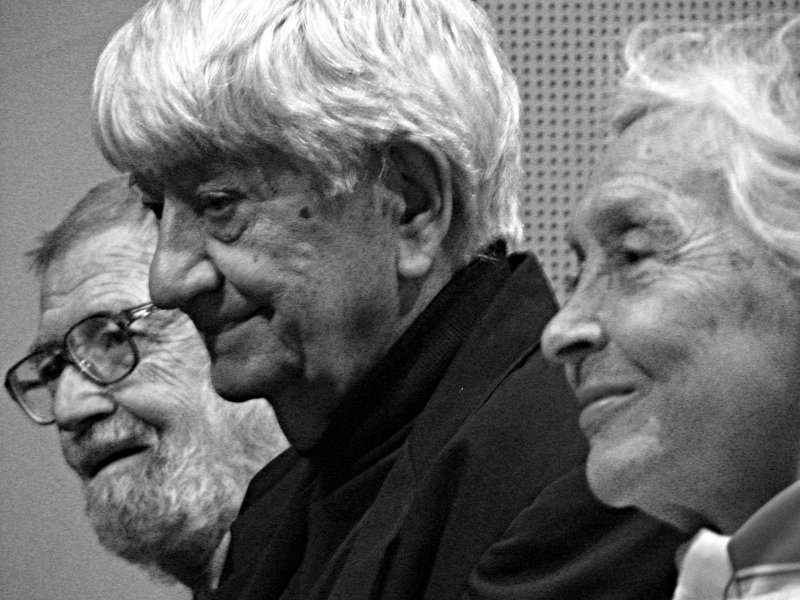
\includegraphics[width=9.2cm]{plavrevue-40/img/vl1.jpg}
 % vl1.jpg: 1179666x1179666 pixel, 0dpi, infxinf cm, bb=
\end{center}
